\documentclass[thesis]{subfiles}

\begin{document}

\OnlyInSubfile{\setcounter{chapter}{3}}

\chapter{Quantum simulations}
\startcontents[chapters]
\printpartialtoc

\section{From Schrödinger equation to Density Functional Theory}

If we want to be able to compute properties of an atomic system using the
framework of statistical physics, we need to be able to compute the total energy
of this system in a given configuration. It is possible to do so by considering
the quantum nature of the atoms, and solving the the Schrödinger equation for
this system. While solving the Schrödinger equation is relatively costly ---
even with the methods presented here --- it present the advantage that no
additional hypothesis has to be done on the system, and the functional form of
the interaction potential $\mathcal{V}(\r^N)$.

In this chapter, I will present the Density Functional Theory approach to
solving the Schrödinger equation, and use it in conjunction with molecular
dynamics to study deformations of \ZIF8 under \ce{N2} adsorption.

\newpage
\subsection{Quantum chemistry and Schrödinger equation}

In the quantum chemistry, the state of a system is represented by a
complex-valued function of positions and time $\Psi(\r, t)$.  The Schrödinger
equation describes the time evolution of this function given the Hamiltonian
$\hat{\mathcal{H}}$ of the system:
\[\hat{\mathcal{H}} \Psi(\r, t) = i\hbar \frac{\partial}{\partial t} \Psi(\r, t),\label{eq:time-schrodinger}\]
where $i$ is the imaginary number, and $\hbar$ the reduced Plank's constant. The
quantum Hamiltonian operator can be expressed as a sum of quantum kinetic energy
and potential energy:
\[\hat{\mathcal{H}} = \sum_i \frac{- \hbar^2}{2m_i} \nabla_i^2 + V(\r)\]
where the $m$ are the masses of the particles in the system, $\nabla$ is the
differential nabla operator, and $V(\r)$ is the potential energy of the system.
When the potential energy does not depend on time, we can look for solution with
separated variables of the form:
\[\Psi(\r, t) = \psi(\r) \times y(t).\]
Replacing in equation~\eqref{eq:time-schrodinger}, and separating the spatial
and time quantities, we get
\[- \sum \frac{\hbar^2}{2m} \frac{1}{\psi(\r)} \nabla^2 \psi(\r) + V(\r) = i\hbar \frac{1}{y(t)} \frac{\d y(t)}{\d t}.\]
For this equation to stand for all $t$ and all $r$, there must exist a constant
value $E$ such that:
\[\begin{dcases}
    E =& - \sum \frac{\hbar^2}{2m} \frac{1}{\psi(\r)} \nabla^2 \psi(\r) + V(\r) \\
    E =& i\hbar \frac{1}{y(t)} \frac{\d y(t)}{\d t} \\
\end{dcases}\]

Putting everything together, any solution of the general
equation~\eqref{eq:time-schrodinger} can be written as a (potential infinite)
linear combination of special solutions:
\[\Psi(r, t) = \sum_i c_i \ \psi_i(r) \ e^{-i E_i t / \hbar},\]
with $c_i$ being the complex coefficients of the combination; and the $(E_i\ ;\
\psi_i)$ pairs are solutions of the \emph{time-independent} Schrödinger equation:
\[\hat{\mathcal{H}} \psi(r) = E \psi(r).\label{eq:schrodinger}\]
Because the time dependence of $\Psi$ have a wave-like form and because $\Psi$
propagate through space and time, it is often called a \emph{wave function}.

\subsection{Density Functional Theory}

To compute the energy of an atomic system, we need to solve
equation~\eqref{eq:schrodinger} for a collections of $N$ electrons carrying the
negative charge $-e$ and $M$ nuclei carrying the positive charge $e Z_j$
interacting though Coulombic potential. As the electrons are much more
lightweight than the nuclei (an electron is 2000 time lighter than a single
proton), it is customary to work under the Born-Oppenheimer approximation. In
this approximation, the degrees of freedom of electrons and nuclei are
decoupled, and the electrons move much faster than the nuclei. This effectively
means that at a given point in time, the electrons evolve in a constant
electrostatic potential from the fixed nuclei. The corresponding Hamiltonian
(using atomic units, \ie $e^2 / 4\pi\epsilon_0 = 1$; $\hbar = 1$; and
$m_\text{electron} = 1$) is:
\[\hat{\mathcal{H}} = \left[-\frac 1 2 \sum_i^N \nabla^2_i - \sum_i^N \sum_j^M \frac{Z_j}{|\r_i - \r_j|} + \sum_i^N \sum_{j>i}^N \frac{1}{|\r_i - \r_j|} \right]\]
We can rewrite this by defining the potential an electron feels due to the
presence of all the nuclei $V_\text{ext}(r) = -\sum_{j} Z_j / |\r - \r_j|$, and
the electron-electron interaction potential $U(r_i, r_j) = 1 / |\r_i -
\r_j|$:
\[\hat{\mathcal{H}} = \left[-\frac 12\sum_{i=1}^N \nabla^2_i + \sum_{i=1}^N V_\text{ext}(\r_i) + \sum_{i=1}^N \sum_{j>i}^N U(\r_i, \r_j)\right] \]
\[\hat{\mathcal{H}} = \hat T + \hat V_\text{ext} + \hat V_{ee} \label{eq:electronic-hamiltonian}\]
The three terms in the Hamiltonian are the kinetic energy $\hat T$, the total
external potential $\hat V_\text{ext}$, and the electron-electron interaction
potential $\hat V_{ee}$.

The Density Functional Theory (DFT) is a strategy to solve the Schrödinger
equation without having to explicitly determine the wave function $\psi$. It is
based on the fact that the square of the norm of the wave function is the
probability for the system to be in a given state. For a system of electrons
evolving in the fixed potential created by the nuclei, the wave function
$\psi(\{\vec x\}, \{s\})$ depends on the Cartesian coordinates of all the
electrons $\{\vec x\}$ and their spins $\{s\}$. The electronic density $n(\vec
r)$ is the probability to find an electron in small neighboring of $\r$. It
is defined as:
\[n(\r) = N \iiint |\psi(\r, s_1, \vec x_2, s2, \cdots, \vec x_N, s_N)|^2 \ \d \vec x_2 \cdots\d \vec x_N \ \d s_1 \cdots\d s_N \label{eq:electron-density}\]
We also define the two electrons density $n_2(\r_1, \r_2)$, which is the
probability for an electron to be in $\r_1$, while another electron is in
$\r_2$:
\[n_2(\r_1, \r_2) = N \iiint |\psi(\r_1, s_1, \r_2, s_2, \vec x_3, s3, \cdots, \vec x_N, s_N)|^2 \ \d \vec x_3 \cdots\d \vec x_N \ \d s_1 \cdots\d s_N\]

Hohenberg and Kohn showed in 1964 that every electronic density correspond
exactly to one and only one external potential $V_\text{ext}$, \ie the knowledge
of the external potential or the density are equivalent. This also means that
knowing the electronic density is equivalent to knowing the wave function of the
system, as one can reconstruct it using equation~\eqref{eq:schrodinger}. As a
consequence, all the observables of the system only depend on the electronic
density, and can be written as functionals of this density: $E[n]$, $\Psi[n]$,
\etc

The second Hohenberg and Kohn theorem states that the ground state electronic
density $n_0(\r)$ is the one that minimize the energy functional: $E[n] \geq
E_0 = E[n_0]$. From the previous relations, the total energy functional contains
three terms:
\[E[n] = T[n] + V_\text{ext}[n] + V_{ee}[n];\]
where the potential terms can be expressed as integrals of the one and two
electrons density:
\[ V_\text{ext}[n] = \int V_\text{ext}(\r) \ n(\r) \ \d \r;\]
\[ V_{ee}[n] = \iint \frac{n_2(\r_1, \r_2)}{|\r_1 - \r_2|} \ \d \r_1 \d \r_2.\]
While we can compute and minimize $V_\text{ext}[n]$ given the positions of the
nuclei, the two other terms are harder to evaluate.

Kohn and Sham reformulated the problem in 1965 by considering a set of
\emph{non-interacting} electrons evolving in a specific external potential, such
as the density arising from these electrons is the same as the one we look for.
The new system of non-interacting electrons is described by a new set of
independent orbitals $\phi_i$, such as the total electronic density of the system
\[n(\r) = \sum_i^N \left| \phi_i(\r) \right|^2\]

For these non interacting electrons, the kinetic energy $T_s[n]$ is known:
\[T_s[n] = \sum_i^N \int \phi_i^*(\r) \left( -\frac 12 \nabla^2 \right) \phi_i(\r) \d \r\]
We also know that most of the electron-electron interactions will arise from the
classical Coulombic interaction --- the Hartree energy --- which we can compute
from the electronic density:
\[V_H[n] = \iint \frac{n(\r_1) n(\r_2)}{|\r_1 - \r_2|} \ \d \r_1 \d \r_2.\]
The functional to minimize in order to find the electronic density is now
\[E[n] = T_s[n] + V_\text{ext}[n] + V_H[n] + E_{xc}[n],\label{eq:energy-functional}\]
in which we can compute all of the terms expect for the exchange-correlation
contribution $E_{xc}[n]$.
\[E_{xc}[n] = (T[n] - T_s[n]) + (V_{ee}[n] - V_H[n]).\]
This contribution is generally unknown, and describe the quantum nature of
electrons that are able to interact with themselves. The exchange-correlation
name comes from the two terms it describe. The exchange energy is a quantum only
effect due to the fact that electrons are not distinguishable, and that
exchanging two of them should change the sign of the wave function. This
exchange effect is sometimes called Pauli repulsion, as it increases the
distance between the electrons. The correlation term describes how much the
presence of other electrons influences the position of a given electron; \ie how
much the two electrons density $n_2(\r_1, \r_2)$ differs from the product of
single electrons densities $n(\r_1)n(\r_2)$.

It can be shown that the minimizing the energy functional is equivalent to
solving a set of differential equations called the Kohn-Sham equations:
\[ \left[-\frac 12 \nabla^2 + V_\text{ext}(\r) + \frac{\partial V_H[n](\r)}{\partial n(\vec r)} + \frac{\partial E_{xc}[n](\r)}{\partial n(\vec r)} \right] \phi_i = \epsilon_i \phi_i \label{eq:kohn-sham}\]
These are non-linear equations, as both $V_H[n]$ and $E_{xc}[n]$ depends on the
$\phi_i$ through $n(\r)$. The usual algorithm to solve them is a self-consistent
iterative algorithm. Starting from an initial guess for the Kohn-Sham orbitals
$\phi_i^0$:
\begin{enumerate}
    \item Calculate the corresponding electron density at step $\alpha$, $n^\alpha(\r)$;
    \item Calculate all the terms in the left hand side of equation~\eqref{eq:kohn-sham}:
          kinetic, external, Hartree and exchange-correlation energies using this electron density;
    \item Solve the Kohn-Sham equation to find new Kohn-Sham orbitals $\phi_i^{\alpha+1}$;
    \item Compute the new energy using the energy functional~\eqref{eq:energy-functional}.
          If this energy is the same as the one in the previous step, then we have found
          the minimal energy and thus the ground state density. Else, go back to step
          1 using the new Kohn-Sham orbitals as the initial guess.
\end{enumerate}

\subsection{Exchange, Correlation and dispersion}

A good approximation for the exchange-correlation functional is required to
solve the Kohn-Sham equations. There are number of approach routinely used in
theoretical chemistry such as Local Density Approximation (LDA) where the
exchange-correlation functional only depends on the local density; Generalized
Gradient Approximation (GGA), where the functional also depends on the local
gradient of the density, meta-GGA functional incorporating the second derivative
of the density (the Laplacian of the density); or hybrid functional. Hybrid
functionals mix exchange expressions from LDA or GGA with more precise
expressions coming from other methods for solving the Schrödinger equation, such
as Hartree-Fock methods.\cite{TODO}

Generally, the exchange-correlation functional only depends on the local
density, and maybe some of its derivative. This means that the DFT method will
have trouble reproducing the non-electrostatic long-range correlation effects
such as the dispersion interaction. Fortunately, we have a simple analytic
formulation for these interaction, which Grimme and coworkers\cite{Grimme2006}
proposed to include when computing the total energy. This correction is added to
the energy obtained by DFT, and does not directly modify the electronic density.
\[E_\text{tot} = E_\text{DFT} + E_\text{disp}; \]
This correction is added to the energy obtained by DFT, and does not directly
modify the electronic density.
\[\text{with}\quad E_\text{disp} = - s_6 \sum_i^M\sum_{j>i}^M\frac{\sqrt{C_6^i C_6^j}}{R_{ij}^6} f_{ij}(R_{ij}),\]
where the sum is over all the pairs of atoms, $R_{ij}$ is the distance between
the atoms, $s_6$ a parameter specifically adapted to the exchange-correlation
functional one uses, the $C_6^i$ are parameters tabulated for each element and
$f_{ij}$ is a damping function.
\[f_{ij}(R_{ij}) =
\begin{dcases}
    \frac{1}{1 + \exp\left[-d \left(R_{ij} / (\sigma_i + \sigma_j) -1\right)\right]} &\text{for } R_{ij} < R_c \\
    0 &\text{for } R_{ij} \geq R_c \\
\end{dcases}\]
In this expression, $d$ is a damping parameter, usually set to 20, $R_c$ a
cutoff radius, and the $\sigma_i$ parameters are tabulated atomic \vdW radii.

\clearpage
\section{Adsorption of \ce{N2} in \ZIF8 and derivatives}

\subsection{\ZIF8 and its cousins}

\ZIF8 is a MOF in the Zeolitic Imidazolate Framework (ZIF) family. ZIFs are
built around tetravalent metal centers such as Fe, Co, Zn or Cu; linked together
by imidazolate linkers. They also present the same topology as zeolites, with
Metal-(imidazolate)$_2$ building blocks taking the role of \ce{SiO2}. The first
ZIFs (ZIF-1 to ZIF-12) were synthesized in 2006\cite{Park2006}, and found to be
water and thermally resistant, which made them interesting MOF for commercial
applications. \ZIF8 --- represented in figure~\ref{fig:zif8-ch3:structure} ---
have a sodalite (SOD) topology, and is composed of methyl-imidazolate linkers
around Zinc metallic centers.

\begin{figure}[ht]
    \centering
    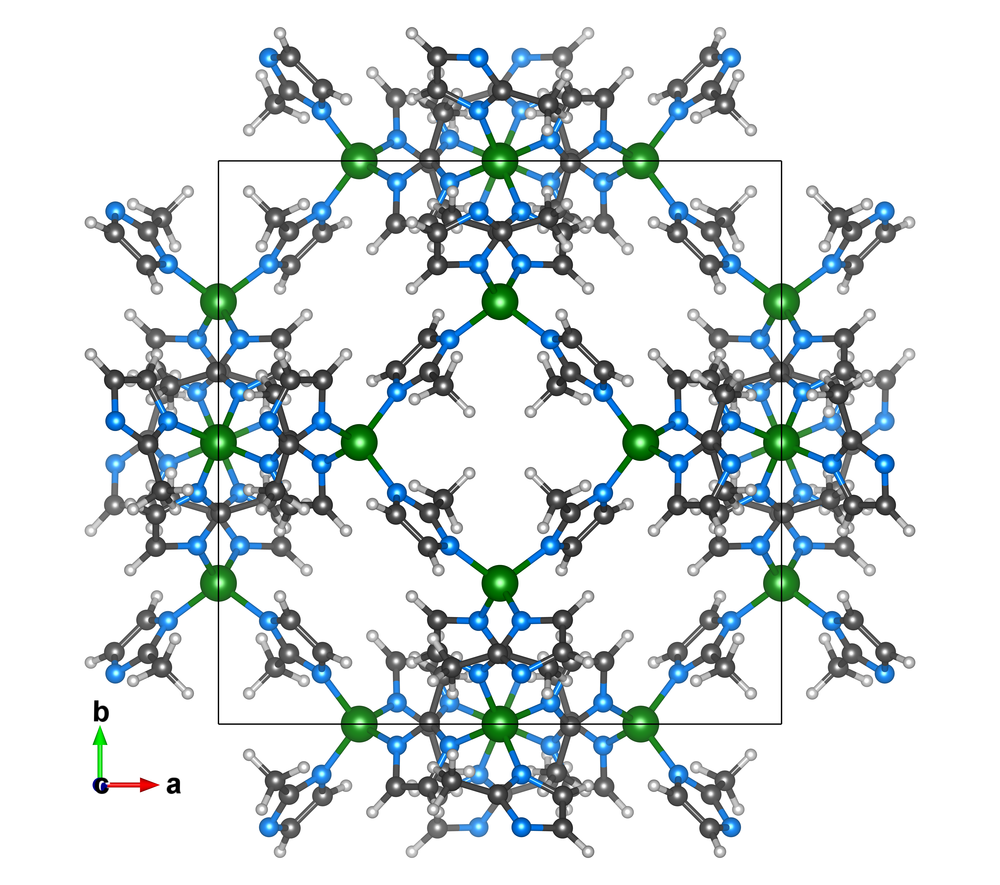
\includegraphics[width=0.35\textwidth]{figures/images/ZIF8-100}
    \hspace{2em}
    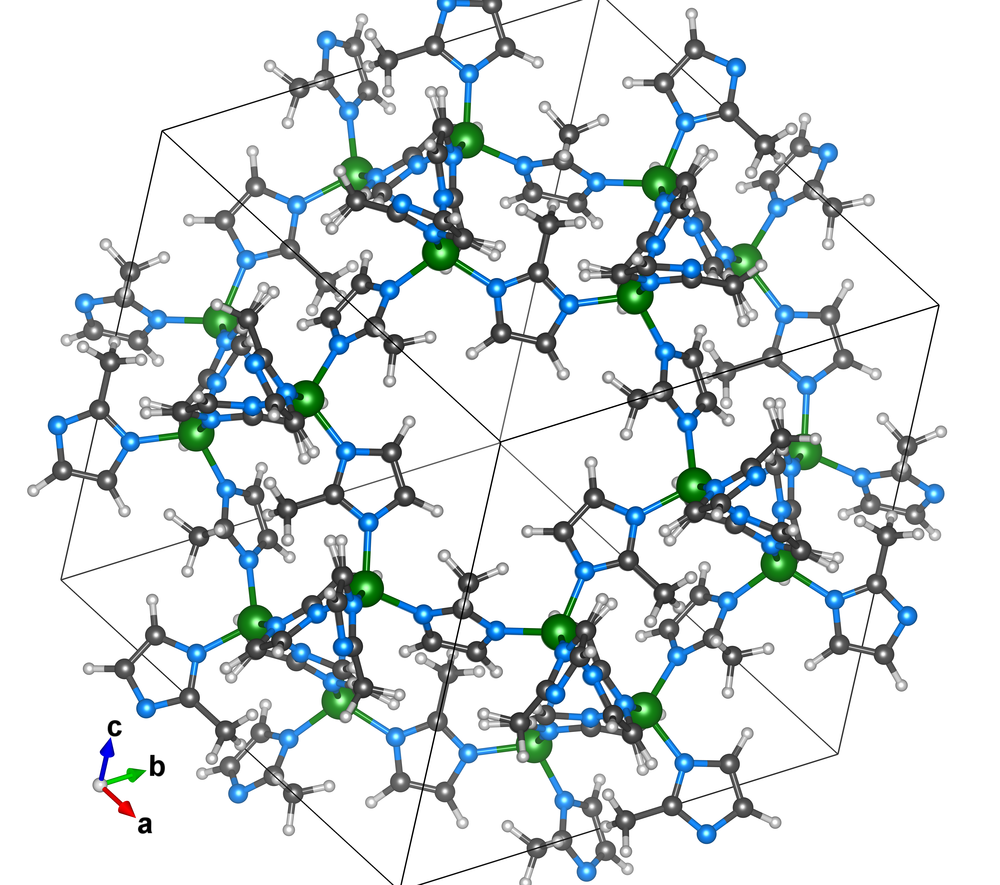
\includegraphics[width=0.35\textwidth]{figures/images/ZIF8-111}
    \caption{Structure of the methyl-imidazolate \ZIF8. On the left, the
    front-most opening is the 4-member ring window (the structure is represented
    along the 001 axis); and on the right the front-most opening is the 6-member
    ring window (the structure is represented along the 111 axis). The atomic
    color code is green for Zinc, blue for Nitrogen, gray for Carbon and white
    for Hydrogen.}
    \label{fig:zif8-ch3:structure}
\end{figure}

Two analogs to \ZIF8 using chloro- and bromo- substituted imidazolate instead of
the original methyl-imidazolate in \ZIF8 have first synthesized by
\citeauthor{Li2009}\cite{Li2009}. These two new materials that we will call
\ZIFCl and \ZIFBr are represented in figure~\ref{fig:zif8-x:structures}.

\begin{figure}[ht]
    \centering
    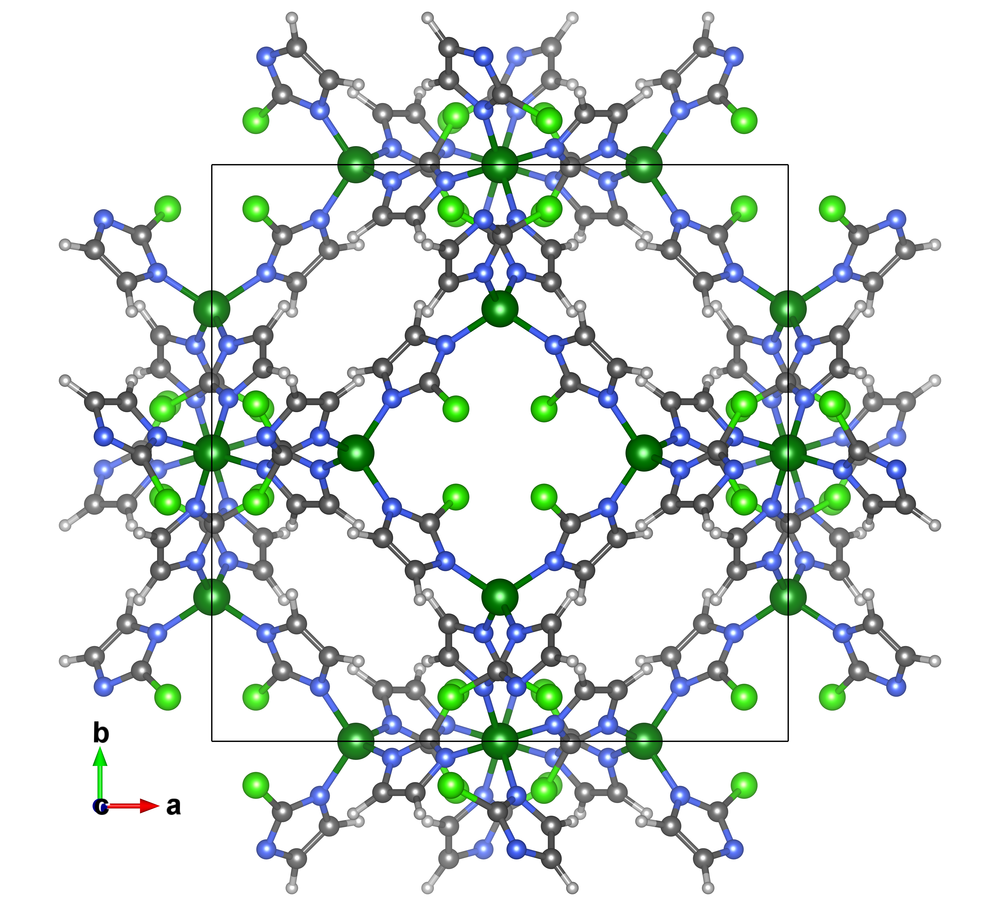
\includegraphics[width=0.35\textwidth]{figures/images/ZIF8-Cl}
    \hspace{2em}
    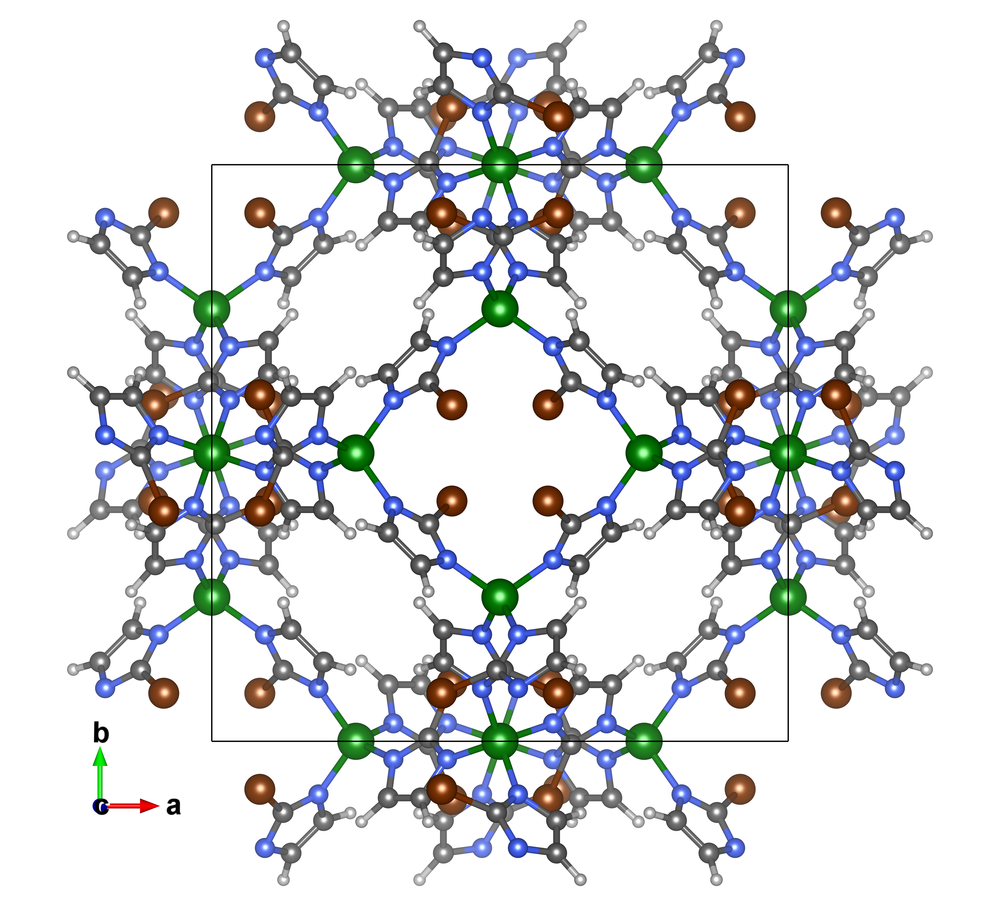
\includegraphics[width=0.35\textwidth]{figures/images/ZIF8-Br}
    \caption{Structure of the chloro-imidazolate \ZIFCl on the left and the
    bromo-imidazolate \ZIFBr on the right. The atomic color code is the same
    as in figure~\ref{fig:zif8-ch3:structure}, with a bright green for Chlorine
    atoms and dark red for Bromide atoms.}
    \label{fig:zif8-x:structures}
\end{figure}

As we will see in this chapter, these simple changes of linker are followed by
complex changes in behavior; showing in this specific example the versatility
MOFs can achieve through organic chemistry.

\FloatBarrier
\subsection{Adsorption isotherms of \ce{N2} in \ZIF8}

\ZIF8 is known for it relatively high surface area of \SI{1.947}{m^2/g} and
large cavity with a diameter of \SI{11.6}{\AA}\cite{Park2006}. It is also
commercially available and have excellent performance at the lab scale for the
separation of gas mixtures such as \ce{C2}/\ce{C3} hydrocarbons,
\ce{CO2}/\ce{CH4}, or \ce{CO2}/\ce{N2}\cite{Li2009,Bux2011}. It also present an
interesting behavior with respect to flexibility of the structure during
nitrogen adsorption. The nitrogen adsorption isotherms at \SI{77}{K} in \ZIF8,
\ZIFCl and \ZIFBr, are presented in figure~\ref{fig:zif8x:isotherms}

\begin{figure}[ht]
    \centering
    % GNUPLOT: LaTeX picture with Postscript
\begingroup
  \makeatletter
  \providecommand\color[2][]{%
    \GenericError{(gnuplot) \space\space\space\@spaces}{%
      Package color not loaded in conjunction with
      terminal option `colourtext'%
    }{See the gnuplot documentation for explanation.%
    }{Either use 'blacktext' in gnuplot or load the package
      color.sty in LaTeX.}%
    \renewcommand\color[2][]{}%
  }%
  \providecommand\includegraphics[2][]{%
    \GenericError{(gnuplot) \space\space\space\@spaces}{%
      Package graphicx or graphics not loaded%
    }{See the gnuplot documentation for explanation.%
    }{The gnuplot epslatex terminal needs graphicx.sty or graphics.sty.}%
    \renewcommand\includegraphics[2][]{}%
  }%
  \providecommand\rotatebox[2]{#2}%
  \@ifundefined{ifGPcolor}{%
    \newif\ifGPcolor
    \GPcolortrue
  }{}%
  \@ifundefined{ifGPblacktext}{%
    \newif\ifGPblacktext
    \GPblacktextfalse
  }{}%
  % define a \g@addto@macro without @ in the name:
  \let\gplgaddtomacro\g@addto@macro
  % define empty templates for all commands taking text:
  \gdef\gplbacktext{}%
  \gdef\gplfronttext{}%
  \makeatother
  \ifGPblacktext
    % no textcolor at all
    \def\colorrgb#1{}%
    \def\colorgray#1{}%
  \else
    % gray or color?
    \ifGPcolor
      \def\colorrgb#1{\color[rgb]{#1}}%
      \def\colorgray#1{\color[gray]{#1}}%
      \expandafter\def\csname LTw\endcsname{\color{white}}%
      \expandafter\def\csname LTb\endcsname{\color{black}}%
      \expandafter\def\csname LTa\endcsname{\color{black}}%
      \expandafter\def\csname LT0\endcsname{\color[rgb]{1,0,0}}%
      \expandafter\def\csname LT1\endcsname{\color[rgb]{0,1,0}}%
      \expandafter\def\csname LT2\endcsname{\color[rgb]{0,0,1}}%
      \expandafter\def\csname LT3\endcsname{\color[rgb]{1,0,1}}%
      \expandafter\def\csname LT4\endcsname{\color[rgb]{0,1,1}}%
      \expandafter\def\csname LT5\endcsname{\color[rgb]{1,1,0}}%
      \expandafter\def\csname LT6\endcsname{\color[rgb]{0,0,0}}%
      \expandafter\def\csname LT7\endcsname{\color[rgb]{1,0.3,0}}%
      \expandafter\def\csname LT8\endcsname{\color[rgb]{0.5,0.5,0.5}}%
    \else
      % gray
      \def\colorrgb#1{\color{black}}%
      \def\colorgray#1{\color[gray]{#1}}%
      \expandafter\def\csname LTw\endcsname{\color{white}}%
      \expandafter\def\csname LTb\endcsname{\color{black}}%
      \expandafter\def\csname LTa\endcsname{\color{black}}%
      \expandafter\def\csname LT0\endcsname{\color{black}}%
      \expandafter\def\csname LT1\endcsname{\color{black}}%
      \expandafter\def\csname LT2\endcsname{\color{black}}%
      \expandafter\def\csname LT3\endcsname{\color{black}}%
      \expandafter\def\csname LT4\endcsname{\color{black}}%
      \expandafter\def\csname LT5\endcsname{\color{black}}%
      \expandafter\def\csname LT6\endcsname{\color{black}}%
      \expandafter\def\csname LT7\endcsname{\color{black}}%
      \expandafter\def\csname LT8\endcsname{\color{black}}%
    \fi
  \fi
    \setlength{\unitlength}{0.0500bp}%
    \ifx\gptboxheight\undefined%
      \newlength{\gptboxheight}%
      \newlength{\gptboxwidth}%
      \newsavebox{\gptboxtext}%
    \fi%
    \setlength{\fboxrule}{0.5pt}%
    \setlength{\fboxsep}{1pt}%
\begin{picture}(5660.00,4240.00)%
    \gplgaddtomacro\gplbacktext{%
      \csname LTb\endcsname%%
      \put(752,694){\makebox(0,0)[r]{\strut{}$0$}}%
      \csname LTb\endcsname%%
      \put(752,1434){\makebox(0,0)[r]{\strut{}$100$}}%
      \csname LTb\endcsname%%
      \put(752,2173){\makebox(0,0)[r]{\strut{}$200$}}%
      \csname LTb\endcsname%%
      \put(752,2913){\makebox(0,0)[r]{\strut{}$300$}}%
      \csname LTb\endcsname%%
      \put(752,3652){\makebox(0,0)[r]{\strut{}$400$}}%
      \csname LTb\endcsname%%
      \put(1533,477){\makebox(0,0){\strut{}$10^{-4}$}}%
      \csname LTb\endcsname%%
      \put(2486,477){\makebox(0,0){\strut{}$10^{-3}$}}%
      \csname LTb\endcsname%%
      \put(3439,477){\makebox(0,0){\strut{}$10^{-2}$}}%
      \csname LTb\endcsname%%
      \put(4392,477){\makebox(0,0){\strut{}$10^{-1}$}}%
    }%
    \gplgaddtomacro\gplfronttext{%
      \csname LTb\endcsname%%
      \put(178,2358){\rotatebox{-270}{\makebox(0,0){\strut{}uptake (\si{cm^3/cm^3} STP)}}}%
      \csname LTb\endcsname%%
      \put(3086,152){\makebox(0,0){\strut{}$P / P_0$}}%
      \csname LTb\endcsname%%
      \put(4518,2249){\makebox(0,0)[r]{\strut{}\footnotesize\ZIFCH3}}%
      \csname LTb\endcsname%%
      \put(4518,2032){\makebox(0,0)[r]{\strut{}\footnotesize\ZIFCl}}%
      \csname LTb\endcsname%%
      \put(4518,1815){\makebox(0,0)[r]{\strut{}\footnotesize\ZIFBr}}%
    }%
    \gplbacktext
    \put(0,0){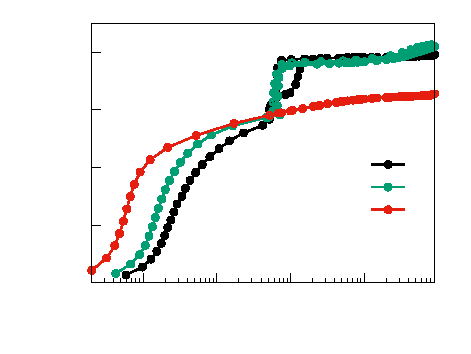
\includegraphics{zif8x-isotherms}}%
    \gplfronttext
  \end{picture}%
\endgroup

    \caption{Adsorption isotherms in \ZIF8 (black) and the chloro (green) and
    bromo (red) derivatives. Full circles are used for the adsorption branch,
    and empty ones for the desorption branch. Experimental data acquired by
    \citeauthor{Chaplais2018}\cite{Chaplais2018}}
    \label{fig:zif8x:isotherms}
\end{figure}

Looking at these isotherms, we first notice that for \ZIF8, there are two jumps
in loading: a first one corresponding to the initial filling of the pores up
until around \SI{300}{cm^3/cm^3}, and the a second one up until
\SI{400}{cm^3/cm^3}. \ZIFCl shows the same behavior with a two stepped isotherm,
while \ZIFBr does not. The adsorption of nitrogen molecules at low temperature
in \ZIF8 has already been studied extensively, both experimentally and by
computational means. Early work demonstrated that the structure of \ZIF8 goes
through at least two phases during the adsorption: an ambient pressure phase
named AP, and a high pressure phase named HP. These phases mainly differ by the
orientation of the linkers around the 4 and 6-member
windows.\cite{FairenJimenez2011} A recent, more detailed characterization of the
structural evolution upon adsorption showed that the transition from AP to HP is
linked to a continuous swing (rotation) of the methyl-imidazolate linker, which
can be followed as the dihedral angle Zn-Zn-C-CH3 goes from an equilibrium value
of 7° in AP phase to an equilibrium value of 35° in HP phase.\cite{Coudert2017}
All this seems to indicate that the second jump in the isotherm is related to
the changes in the structure.

In order to gain better understanding of the relation between the structure
changes and the adsorbed molecules, I used molecular dynamics (MD) simulations.
To describe fully the flexibility of the frameworks without any assumption, I
favored \abinitio MD over force field-based MD --- as there are currently no
force fields available for the \ZIF8 variants studied here. For each framework
(\ZIF8(\ce{CH3}), \ZIFCl, \ZIFBr), I ran five simulations corresponding to
different number of nitrogen molecules inside the porous space, going from empty
framework ($N = 0$) to the fully loaded host material. The maximal loading was
determined from the experimental isotherms to be close to $N = 50$ molecules per
unit cell for \ZIF8(\ce{CH3}) and \ZIFCl and $N = 40$ molecules per unit cell
for \ZIFBr.

To create the starting configurations, I started from the energy-minimized
configuration of the empty frameworks, and randomly placed the selected number
of nitrogen molecules in the unit cell using the packmol
software\cite{Martnez2009}.  The whole \{ZIF, adsorbate\} system was then
minimized again before starting the molecular dynamics simulations. I used the
Quickstep module\cite{VandeVondele2005} of the CP2K software package (version
2.5.1, available online at http://www.cp2k.org/) for all the simulations. I used
a PBE exchange-correlation functional with D3 dispersion corrections, a double
zeta polarizable valence (DZVP) basis set, and an energetic cutoff of 600 Ry.
All the systems were simulated with a \SI{1}{fs} timestep giving a total of 12
to \SI{22}{ps} of simulation. Temperature was held constant at 77 K with a CVSR
thermostat, using a thermostat time constant of \SI{1000}{fs}. I used the last
\SI{5}{ps} of simulation for analysis, leaving 7 to \SI{17}{ps} to the system to
reach equilibrium.

\subsection{Deformation under adsorption}

The first indicator of deformation of the framework is the \ce{Zn-Zn-Zn-X}
dihedral angle, where \ce{X} is the group on the imidazolate linkers: methyl,
chlorine or bromide. This angle --- represented on
figure~\ref{fig:zif8x:swing-angle} --- is also called the swing angle.

\begin{figure}[ht]
    \centering
    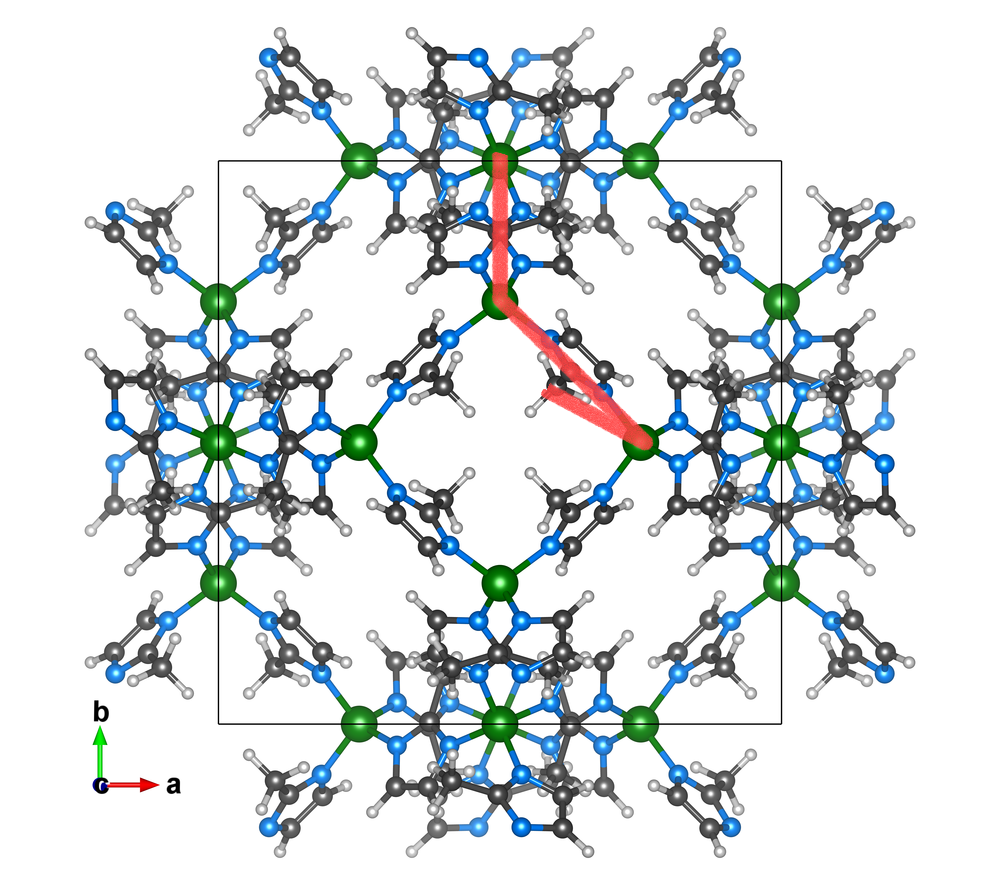
\includegraphics[width=0.3\textwidth]{figures/images/swing-angle}
    \caption{Representation of the swing \ce{Zn-Zn-Zn-X} dihedral angle for \ZIF8.}
    \label{fig:zif8x:swing-angle}
\end{figure}

\begin{figure}[ht]
    \centering
    % GNUPLOT: LaTeX picture with Postscript
\begingroup
  \makeatletter
  \providecommand\color[2][]{%
    \GenericError{(gnuplot) \space\space\space\@spaces}{%
      Package color not loaded in conjunction with
      terminal option `colourtext'%
    }{See the gnuplot documentation for explanation.%
    }{Either use 'blacktext' in gnuplot or load the package
      color.sty in LaTeX.}%
    \renewcommand\color[2][]{}%
  }%
  \providecommand\includegraphics[2][]{%
    \GenericError{(gnuplot) \space\space\space\@spaces}{%
      Package graphicx or graphics not loaded%
    }{See the gnuplot documentation for explanation.%
    }{The gnuplot epslatex terminal needs graphicx.sty or graphics.sty.}%
    \renewcommand\includegraphics[2][]{}%
  }%
  \providecommand\rotatebox[2]{#2}%
  \@ifundefined{ifGPcolor}{%
    \newif\ifGPcolor
    \GPcolortrue
  }{}%
  \@ifundefined{ifGPblacktext}{%
    \newif\ifGPblacktext
    \GPblacktextfalse
  }{}%
  % define a \g@addto@macro without @ in the name:
  \let\gplgaddtomacro\g@addto@macro
  % define empty templates for all commands taking text:
  \gdef\gplbacktext{}%
  \gdef\gplfronttext{}%
  \makeatother
  \ifGPblacktext
    % no textcolor at all
    \def\colorrgb#1{}%
    \def\colorgray#1{}%
  \else
    % gray or color?
    \ifGPcolor
      \def\colorrgb#1{\color[rgb]{#1}}%
      \def\colorgray#1{\color[gray]{#1}}%
      \expandafter\def\csname LTw\endcsname{\color{white}}%
      \expandafter\def\csname LTb\endcsname{\color{black}}%
      \expandafter\def\csname LTa\endcsname{\color{black}}%
      \expandafter\def\csname LT0\endcsname{\color[rgb]{1,0,0}}%
      \expandafter\def\csname LT1\endcsname{\color[rgb]{0,1,0}}%
      \expandafter\def\csname LT2\endcsname{\color[rgb]{0,0,1}}%
      \expandafter\def\csname LT3\endcsname{\color[rgb]{1,0,1}}%
      \expandafter\def\csname LT4\endcsname{\color[rgb]{0,1,1}}%
      \expandafter\def\csname LT5\endcsname{\color[rgb]{1,1,0}}%
      \expandafter\def\csname LT6\endcsname{\color[rgb]{0,0,0}}%
      \expandafter\def\csname LT7\endcsname{\color[rgb]{1,0.3,0}}%
      \expandafter\def\csname LT8\endcsname{\color[rgb]{0.5,0.5,0.5}}%
    \else
      % gray
      \def\colorrgb#1{\color{black}}%
      \def\colorgray#1{\color[gray]{#1}}%
      \expandafter\def\csname LTw\endcsname{\color{white}}%
      \expandafter\def\csname LTb\endcsname{\color{black}}%
      \expandafter\def\csname LTa\endcsname{\color{black}}%
      \expandafter\def\csname LT0\endcsname{\color{black}}%
      \expandafter\def\csname LT1\endcsname{\color{black}}%
      \expandafter\def\csname LT2\endcsname{\color{black}}%
      \expandafter\def\csname LT3\endcsname{\color{black}}%
      \expandafter\def\csname LT4\endcsname{\color{black}}%
      \expandafter\def\csname LT5\endcsname{\color{black}}%
      \expandafter\def\csname LT6\endcsname{\color{black}}%
      \expandafter\def\csname LT7\endcsname{\color{black}}%
      \expandafter\def\csname LT8\endcsname{\color{black}}%
    \fi
  \fi
    \setlength{\unitlength}{0.0500bp}%
    \ifx\gptboxheight\undefined%
      \newlength{\gptboxheight}%
      \newlength{\gptboxwidth}%
      \newsavebox{\gptboxtext}%
    \fi%
    \setlength{\fboxrule}{0.5pt}%
    \setlength{\fboxsep}{1pt}%
\begin{picture}(7760.00,3100.00)%
    \gplgaddtomacro\gplbacktext{%
      \csname LTb\endcsname%%
      \put(212,341){\makebox(0,0){\strut{}$0$}}%
      \csname LTb\endcsname%%
      \put(636,341){\makebox(0,0){\strut{}$10$}}%
      \csname LTb\endcsname%%
      \put(1060,341){\makebox(0,0){\strut{}$20$}}%
      \csname LTb\endcsname%%
      \put(1483,341){\makebox(0,0){\strut{}$30$}}%
      \csname LTb\endcsname%%
      \put(1907,341){\makebox(0,0){\strut{}$40$}}%
      \csname LTb\endcsname%%
      \put(2331,341){\makebox(0,0){\strut{}$50$}}%
    }%
    \gplgaddtomacro\gplfronttext{%
      \csname LTb\endcsname%%
      \put(1271,109){\makebox(0,0){\strut{}$\phi$ (°)}}%
      \csname LTb\endcsname%%
      \put(1271,2867){\makebox(0,0){\strut{}\ZIFCH3}}%
      \csname LTb\endcsname%%
      \put(1759,2494){\makebox(0,0)[r]{\strut{}\scriptsize 0 \ce{N2}}}%
      \csname LTb\endcsname%%
      \put(1759,2339){\makebox(0,0)[r]{\strut{}\scriptsize 10 \ce{N2}}}%
      \csname LTb\endcsname%%
      \put(1759,2184){\makebox(0,0)[r]{\strut{}\scriptsize 25 \ce{N2}}}%
      \csname LTb\endcsname%%
      \put(1759,2029){\makebox(0,0)[r]{\strut{}\scriptsize 40 \ce{N2}}}%
      \csname LTb\endcsname%%
      \put(1759,1874){\makebox(0,0)[r]{\strut{}\scriptsize 50 \ce{N2}}}%
    }%
    \gplgaddtomacro\gplbacktext{%
      \csname LTb\endcsname%%
      \put(2628,341){\makebox(0,0){\strut{}$0$}}%
      \csname LTb\endcsname%%
      \put(3086,341){\makebox(0,0){\strut{}$10$}}%
      \csname LTb\endcsname%%
      \put(3544,341){\makebox(0,0){\strut{}$20$}}%
      \csname LTb\endcsname%%
      \put(4001,341){\makebox(0,0){\strut{}$30$}}%
      \csname LTb\endcsname%%
      \put(4459,341){\makebox(0,0){\strut{}$40$}}%
      \csname LTb\endcsname%%
      \put(4917,341){\makebox(0,0){\strut{}$50$}}%
    }%
    \gplgaddtomacro\gplfronttext{%
      \csname LTb\endcsname%%
      \put(3772,109){\makebox(0,0){\strut{}$\phi$ (°)}}%
      \csname LTb\endcsname%%
      \put(3772,2867){\makebox(0,0){\strut{}\ZIFCl}}%
      \csname LTb\endcsname%%
      \put(4345,2494){\makebox(0,0)[r]{\strut{}\scriptsize 0 \ce{N2}}}%
      \csname LTb\endcsname%%
      \put(4345,2339){\makebox(0,0)[r]{\strut{}\scriptsize 10 \ce{N2}}}%
      \csname LTb\endcsname%%
      \put(4345,2184){\makebox(0,0)[r]{\strut{}\scriptsize 25 \ce{N2}}}%
      \csname LTb\endcsname%%
      \put(4345,2029){\makebox(0,0)[r]{\strut{}\scriptsize 40 \ce{N2}}}%
      \csname LTb\endcsname%%
      \put(4345,1874){\makebox(0,0)[r]{\strut{}\scriptsize 50 \ce{N2}}}%
    }%
    \gplgaddtomacro\gplbacktext{%
      \csname LTb\endcsname%%
      \put(5215,341){\makebox(0,0){\strut{}$0$}}%
      \csname LTb\endcsname%%
      \put(5673,341){\makebox(0,0){\strut{}$10$}}%
      \csname LTb\endcsname%%
      \put(6131,341){\makebox(0,0){\strut{}$20$}}%
      \csname LTb\endcsname%%
      \put(6588,341){\makebox(0,0){\strut{}$30$}}%
      \csname LTb\endcsname%%
      \put(7046,341){\makebox(0,0){\strut{}$40$}}%
      \csname LTb\endcsname%%
      \put(7504,341){\makebox(0,0){\strut{}$50$}}%
    }%
    \gplgaddtomacro\gplfronttext{%
      \csname LTb\endcsname%%
      \put(6359,109){\makebox(0,0){\strut{}$\phi$ (°)}}%
      \csname LTb\endcsname%%
      \put(6359,2867){\makebox(0,0){\strut{}\ZIFBr}}%
      \csname LTb\endcsname%%
      \put(6932,2494){\makebox(0,0)[r]{\strut{}\scriptsize 0 \ce{N2}}}%
      \csname LTb\endcsname%%
      \put(6932,2339){\makebox(0,0)[r]{\strut{}\scriptsize 8 \ce{N2}}}%
      \csname LTb\endcsname%%
      \put(6932,2184){\makebox(0,0)[r]{\strut{}\scriptsize 20 \ce{N2}}}%
      \csname LTb\endcsname%%
      \put(6932,2029){\makebox(0,0)[r]{\strut{}\scriptsize 40 \ce{N2}}}%
      \csname LTb\endcsname%%
      \put(6932,1874){\makebox(0,0)[r]{\strut{}\scriptsize 50 \ce{N2}}}%
    }%
    \gplbacktext
    \put(0,0){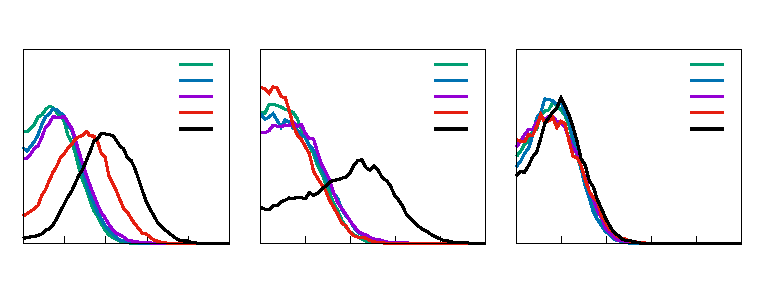
\includegraphics{zif8x-dihedrals}}%
    \gplfronttext
  \end{picture}%
\endgroup

    \caption{Distribution of linker swing angle (\ce{Zn-Zn-Zn-X} dihedral angle,
    where \ce{X} stands for \ce{CH3}, \ce{Cl} or \ce{Br} for \ZIF8, \ZIFCl or
    \ZIFBr, respectively) at various values of nitrogen loading.}
    \label{fig:zif8x:dihedrals}
\end{figure}

Following the evolution of the distributions of angles as the number of nitrogen
molecules increases allow to understand the deformations of the three framework
under adsorption. This evolution is represented on
figure~\ref{fig:zif8x:dihedrals}, where we observe a gradual increase of the
mean angle value as loading increases while the distribution stays Gaussian.

These results are consistent with the already published ones for
\ZIF8\cite{Coudert2017}. Interestingly, the two other frameworks behave
differently. For \ZIFCl, no change is noticed in the distribution profile upon
adsorption until the highest value of loading (\ie, $N = 50$). In this case, the
distribution shifts and the profile is no longer Gaussian type, but instead
looks like the sum of two Gaussian distribution, one centered around 25°, and
the other one around 10°. It indicates that some of the linkers do not rotate
(swing) even at high loading. This non-zero value of the distribution at $\phi =
0\text{°}$ contrasts with the case of \ZIF8. Finally, for \ZIFBr, no change
occurs for the dihedral angle distribution as the loading increases.

Although this behavior is correlated with the presence or absence of the
adsorption step in the isotherms, it is not however sufficient to explain it.
One hypothesis often formulated for \ZIF8 is that the swinging motion leads to
an increase of the accessible porous volume in the structure, thereby increasing
nitrogen uptake. In order to check whether this is or not the case, I computed
the pore size distribution (see figure~\ref{fig:zif8x:pores-sizes}) and the
accessible porous volume (see figure~\ref{fig:zif8x:porous-volume}) from the MD
trajectories using Zeo++\cite{Willems2012} version 0.3. In order to compute
these values, I first emptied the structure of all the nitrogen molecules, and
then computed the pores sizes distribution and accessible volume using the
remaining frameworks.

\begin{figure}[ht]
    \centering
    % GNUPLOT: LaTeX picture with Postscript
\begingroup
  \makeatletter
  \providecommand\color[2][]{%
    \GenericError{(gnuplot) \space\space\space\@spaces}{%
      Package color not loaded in conjunction with
      terminal option `colourtext'%
    }{See the gnuplot documentation for explanation.%
    }{Either use 'blacktext' in gnuplot or load the package
      color.sty in LaTeX.}%
    \renewcommand\color[2][]{}%
  }%
  \providecommand\includegraphics[2][]{%
    \GenericError{(gnuplot) \space\space\space\@spaces}{%
      Package graphicx or graphics not loaded%
    }{See the gnuplot documentation for explanation.%
    }{The gnuplot epslatex terminal needs graphicx.sty or graphics.sty.}%
    \renewcommand\includegraphics[2][]{}%
  }%
  \providecommand\rotatebox[2]{#2}%
  \@ifundefined{ifGPcolor}{%
    \newif\ifGPcolor
    \GPcolortrue
  }{}%
  \@ifundefined{ifGPblacktext}{%
    \newif\ifGPblacktext
    \GPblacktextfalse
  }{}%
  % define a \g@addto@macro without @ in the name:
  \let\gplgaddtomacro\g@addto@macro
  % define empty templates for all commands taking text:
  \gdef\gplbacktext{}%
  \gdef\gplfronttext{}%
  \makeatother
  \ifGPblacktext
    % no textcolor at all
    \def\colorrgb#1{}%
    \def\colorgray#1{}%
  \else
    % gray or color?
    \ifGPcolor
      \def\colorrgb#1{\color[rgb]{#1}}%
      \def\colorgray#1{\color[gray]{#1}}%
      \expandafter\def\csname LTw\endcsname{\color{white}}%
      \expandafter\def\csname LTb\endcsname{\color{black}}%
      \expandafter\def\csname LTa\endcsname{\color{black}}%
      \expandafter\def\csname LT0\endcsname{\color[rgb]{1,0,0}}%
      \expandafter\def\csname LT1\endcsname{\color[rgb]{0,1,0}}%
      \expandafter\def\csname LT2\endcsname{\color[rgb]{0,0,1}}%
      \expandafter\def\csname LT3\endcsname{\color[rgb]{1,0,1}}%
      \expandafter\def\csname LT4\endcsname{\color[rgb]{0,1,1}}%
      \expandafter\def\csname LT5\endcsname{\color[rgb]{1,1,0}}%
      \expandafter\def\csname LT6\endcsname{\color[rgb]{0,0,0}}%
      \expandafter\def\csname LT7\endcsname{\color[rgb]{1,0.3,0}}%
      \expandafter\def\csname LT8\endcsname{\color[rgb]{0.5,0.5,0.5}}%
    \else
      % gray
      \def\colorrgb#1{\color{black}}%
      \def\colorgray#1{\color[gray]{#1}}%
      \expandafter\def\csname LTw\endcsname{\color{white}}%
      \expandafter\def\csname LTb\endcsname{\color{black}}%
      \expandafter\def\csname LTa\endcsname{\color{black}}%
      \expandafter\def\csname LT0\endcsname{\color{black}}%
      \expandafter\def\csname LT1\endcsname{\color{black}}%
      \expandafter\def\csname LT2\endcsname{\color{black}}%
      \expandafter\def\csname LT3\endcsname{\color{black}}%
      \expandafter\def\csname LT4\endcsname{\color{black}}%
      \expandafter\def\csname LT5\endcsname{\color{black}}%
      \expandafter\def\csname LT6\endcsname{\color{black}}%
      \expandafter\def\csname LT7\endcsname{\color{black}}%
      \expandafter\def\csname LT8\endcsname{\color{black}}%
    \fi
  \fi
    \setlength{\unitlength}{0.0500bp}%
    \ifx\gptboxheight\undefined%
      \newlength{\gptboxheight}%
      \newlength{\gptboxwidth}%
      \newsavebox{\gptboxtext}%
    \fi%
    \setlength{\fboxrule}{0.5pt}%
    \setlength{\fboxsep}{1pt}%
\begin{picture}(7360.00,2820.00)%
    \gplgaddtomacro\gplbacktext{%
      \csname LTb\endcsname%%
      \put(274,341){\makebox(0,0){\strut{}$8$}}%
      \csname LTb\endcsname%%
      \put(755,341){\makebox(0,0){\strut{}$9$}}%
      \csname LTb\endcsname%%
      \put(1236,341){\makebox(0,0){\strut{}$10$}}%
      \csname LTb\endcsname%%
      \put(1717,341){\makebox(0,0){\strut{}$11$}}%
      \csname LTb\endcsname%%
      \put(2198,341){\makebox(0,0){\strut{}$12$}}%
    }%
    \gplgaddtomacro\gplfronttext{%
      \csname LTb\endcsname%%
      \put(42,1425){\rotatebox{-270}{\makebox(0,0){\strut{}\scriptsize pore size distribution (log scale)}}}%
      \csname LTb\endcsname%%
      \put(1236,109){\makebox(0,0){\strut{}\scriptsize pore size (\AA)}}%
      \csname LTb\endcsname%%
      \put(1236,2587){\makebox(0,0){\strut{}\ZIFCH3}}%
      \csname LTb\endcsname%%
      \put(727,2183){\makebox(0,0)[r]{\strut{}\scriptsize 0 \ce{N2}}}%
      \csname LTb\endcsname%%
      \put(727,2028){\makebox(0,0)[r]{\strut{}\scriptsize 10 \ce{N2}}}%
      \csname LTb\endcsname%%
      \put(727,1873){\makebox(0,0)[r]{\strut{}\scriptsize 25 \ce{N2}}}%
      \csname LTb\endcsname%%
      \put(727,1718){\makebox(0,0)[r]{\strut{}\scriptsize 40 \ce{N2}}}%
      \csname LTb\endcsname%%
      \put(727,1563){\makebox(0,0)[r]{\strut{}\scriptsize 50 \ce{N2}}}%
    }%
    \gplgaddtomacro\gplbacktext{%
      \csname LTb\endcsname%%
      \put(2495,341){\makebox(0,0){\strut{}$8$}}%
      \csname LTb\endcsname%%
      \put(3034,341){\makebox(0,0){\strut{}$9$}}%
      \csname LTb\endcsname%%
      \put(3573,341){\makebox(0,0){\strut{}$10$}}%
      \csname LTb\endcsname%%
      \put(4112,341){\makebox(0,0){\strut{}$11$}}%
      \csname LTb\endcsname%%
      \put(4651,341){\makebox(0,0){\strut{}$12$}}%
    }%
    \gplgaddtomacro\gplfronttext{%
      \csname LTb\endcsname%%
      \put(3573,109){\makebox(0,0){\strut{}\scriptsize pore size (\AA)}}%
      \csname LTb\endcsname%%
      \put(3573,2587){\makebox(0,0){\strut{}\ZIFCl}}%
      \csname LTb\endcsname%%
      \put(3040,2183){\makebox(0,0)[r]{\strut{}\scriptsize 0 \ce{N2}}}%
      \csname LTb\endcsname%%
      \put(3040,2028){\makebox(0,0)[r]{\strut{}\scriptsize 10 \ce{N2}}}%
      \csname LTb\endcsname%%
      \put(3040,1873){\makebox(0,0)[r]{\strut{}\scriptsize 25 \ce{N2}}}%
      \csname LTb\endcsname%%
      \put(3040,1718){\makebox(0,0)[r]{\strut{}\scriptsize 40 \ce{N2}}}%
      \csname LTb\endcsname%%
      \put(3040,1563){\makebox(0,0)[r]{\strut{}\scriptsize 50 \ce{N2}2}}%
    }%
    \gplgaddtomacro\gplbacktext{%
      \csname LTb\endcsname%%
      \put(4948,341){\makebox(0,0){\strut{}$8$}}%
      \csname LTb\endcsname%%
      \put(5487,341){\makebox(0,0){\strut{}$9$}}%
      \csname LTb\endcsname%%
      \put(6026,341){\makebox(0,0){\strut{}$10$}}%
      \csname LTb\endcsname%%
      \put(6565,341){\makebox(0,0){\strut{}$11$}}%
      \csname LTb\endcsname%%
      \put(7104,341){\makebox(0,0){\strut{}$12$}}%
    }%
    \gplgaddtomacro\gplfronttext{%
      \csname LTb\endcsname%%
      \put(6026,109){\makebox(0,0){\strut{}\scriptsize pore size (\AA)}}%
      \csname LTb\endcsname%%
      \put(6026,2587){\makebox(0,0){\strut{}\ZIFBr}}%
      \csname LTb\endcsname%%
      \put(5493,2183){\makebox(0,0)[r]{\strut{}\scriptsize 0 \ce{N2}}}%
      \csname LTb\endcsname%%
      \put(5493,2028){\makebox(0,0)[r]{\strut{}\scriptsize 8 \ce{N2}}}%
      \csname LTb\endcsname%%
      \put(5493,1873){\makebox(0,0)[r]{\strut{}\scriptsize 20 \ce{N2}}}%
      \csname LTb\endcsname%%
      \put(5493,1718){\makebox(0,0)[r]{\strut{}\scriptsize 40 \ce{N2}}}%
      \csname LTb\endcsname%%
      \put(5493,1563){\makebox(0,0)[r]{\strut{}\scriptsize 50 \ce{N2}}}%
    }%
    \gplbacktext
    \put(0,0){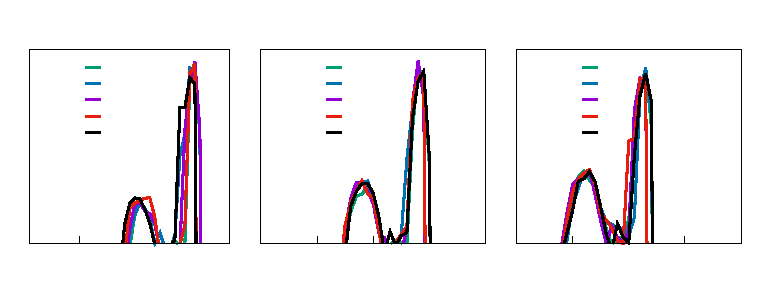
\includegraphics{zif8x-pores-sizes}}%
    \gplfronttext
  \end{picture}%
\endgroup

    \caption{Pore size distribution (no unit) under increasing loading for the
    three structures.}
    \label{fig:zif8x:pores-sizes}
\end{figure}

\begin{figure}[ht]
    \centering
    % GNUPLOT: LaTeX picture with Postscript
\begingroup
  \makeatletter
  \providecommand\color[2][]{%
    \GenericError{(gnuplot) \space\space\space\@spaces}{%
      Package color not loaded in conjunction with
      terminal option `colourtext'%
    }{See the gnuplot documentation for explanation.%
    }{Either use 'blacktext' in gnuplot or load the package
      color.sty in LaTeX.}%
    \renewcommand\color[2][]{}%
  }%
  \providecommand\includegraphics[2][]{%
    \GenericError{(gnuplot) \space\space\space\@spaces}{%
      Package graphicx or graphics not loaded%
    }{See the gnuplot documentation for explanation.%
    }{The gnuplot epslatex terminal needs graphicx.sty or graphics.sty.}%
    \renewcommand\includegraphics[2][]{}%
  }%
  \providecommand\rotatebox[2]{#2}%
  \@ifundefined{ifGPcolor}{%
    \newif\ifGPcolor
    \GPcolortrue
  }{}%
  \@ifundefined{ifGPblacktext}{%
    \newif\ifGPblacktext
    \GPblacktextfalse
  }{}%
  % define a \g@addto@macro without @ in the name:
  \let\gplgaddtomacro\g@addto@macro
  % define empty templates for all commands taking text:
  \gdef\gplbacktext{}%
  \gdef\gplfronttext{}%
  \makeatother
  \ifGPblacktext
    % no textcolor at all
    \def\colorrgb#1{}%
    \def\colorgray#1{}%
  \else
    % gray or color?
    \ifGPcolor
      \def\colorrgb#1{\color[rgb]{#1}}%
      \def\colorgray#1{\color[gray]{#1}}%
      \expandafter\def\csname LTw\endcsname{\color{white}}%
      \expandafter\def\csname LTb\endcsname{\color{black}}%
      \expandafter\def\csname LTa\endcsname{\color{black}}%
      \expandafter\def\csname LT0\endcsname{\color[rgb]{1,0,0}}%
      \expandafter\def\csname LT1\endcsname{\color[rgb]{0,1,0}}%
      \expandafter\def\csname LT2\endcsname{\color[rgb]{0,0,1}}%
      \expandafter\def\csname LT3\endcsname{\color[rgb]{1,0,1}}%
      \expandafter\def\csname LT4\endcsname{\color[rgb]{0,1,1}}%
      \expandafter\def\csname LT5\endcsname{\color[rgb]{1,1,0}}%
      \expandafter\def\csname LT6\endcsname{\color[rgb]{0,0,0}}%
      \expandafter\def\csname LT7\endcsname{\color[rgb]{1,0.3,0}}%
      \expandafter\def\csname LT8\endcsname{\color[rgb]{0.5,0.5,0.5}}%
    \else
      % gray
      \def\colorrgb#1{\color{black}}%
      \def\colorgray#1{\color[gray]{#1}}%
      \expandafter\def\csname LTw\endcsname{\color{white}}%
      \expandafter\def\csname LTb\endcsname{\color{black}}%
      \expandafter\def\csname LTa\endcsname{\color{black}}%
      \expandafter\def\csname LT0\endcsname{\color{black}}%
      \expandafter\def\csname LT1\endcsname{\color{black}}%
      \expandafter\def\csname LT2\endcsname{\color{black}}%
      \expandafter\def\csname LT3\endcsname{\color{black}}%
      \expandafter\def\csname LT4\endcsname{\color{black}}%
      \expandafter\def\csname LT5\endcsname{\color{black}}%
      \expandafter\def\csname LT6\endcsname{\color{black}}%
      \expandafter\def\csname LT7\endcsname{\color{black}}%
      \expandafter\def\csname LT8\endcsname{\color{black}}%
    \fi
  \fi
    \setlength{\unitlength}{0.0500bp}%
    \ifx\gptboxheight\undefined%
      \newlength{\gptboxheight}%
      \newlength{\gptboxwidth}%
      \newsavebox{\gptboxtext}%
    \fi%
    \setlength{\fboxrule}{0.5pt}%
    \setlength{\fboxsep}{1pt}%
\begin{picture}(7360.00,2820.00)%
    \gplgaddtomacro\gplbacktext{%
      \csname LTb\endcsname%%
      \put(622,310){\makebox(0,0)[r]{\strut{}$0$}}%
      \csname LTb\endcsname%%
      \put(622,702){\makebox(0,0)[r]{\strut{}$250$}}%
      \csname LTb\endcsname%%
      \put(622,1095){\makebox(0,0)[r]{\strut{}$500$}}%
      \csname LTb\endcsname%%
      \put(622,1487){\makebox(0,0)[r]{\strut{}$750$}}%
      \csname LTb\endcsname%%
      \put(622,1879){\makebox(0,0)[r]{\strut{}$1000$}}%
      \csname LTb\endcsname%%
      \put(622,2272){\makebox(0,0)[r]{\strut{}$1250$}}%
      \csname LTb\endcsname%%
      \put(622,2664){\makebox(0,0)[r]{\strut{}$1500$}}%
      \csname LTb\endcsname%%
      \put(1773,155){\makebox(0,0){\strut{}\ZIF8}}%
      \csname LTb\endcsname%%
      \put(3906,155){\makebox(0,0){\strut{}\ZIFCl}}%
      \csname LTb\endcsname%%
      \put(6038,155){\makebox(0,0){\strut{}\ZIFBr}}%
      \csname LTb\endcsname%%
      \put(1027,2334){\makebox(0,0)[l]{\strut{}\scriptsize 0}}%
      \csname LTb\endcsname%%
      \put(1347,2350){\makebox(0,0)[l]{\strut{}\scriptsize 10}}%
      \csname LTb\endcsname%%
      \put(1709,2342){\makebox(0,0)[l]{\strut{}\scriptsize 25}}%
      \csname LTb\endcsname%%
      \put(2050,2295){\makebox(0,0)[l]{\strut{}\scriptsize 40}}%
      \csname LTb\endcsname%%
      \put(2413,2256){\makebox(0,0)[l]{\strut{}\scriptsize 50}}%
      \csname LTb\endcsname%%
      \put(3159,2303){\makebox(0,0)[l]{\strut{}\scriptsize 0}}%
      \csname LTb\endcsname%%
      \put(3500,2287){\makebox(0,0)[l]{\strut{}\scriptsize 10}}%
      \csname LTb\endcsname%%
      \put(3842,2311){\makebox(0,0)[l]{\strut{}\scriptsize 25}}%
      \csname LTb\endcsname%%
      \put(4183,2319){\makebox(0,0)[l]{\strut{}\scriptsize 40}}%
      \csname LTb\endcsname%%
      \put(4545,2232){\makebox(0,0)[l]{\strut{}\scriptsize 50}}%
      \csname LTb\endcsname%%
      \put(5292,2138){\makebox(0,0)[l]{\strut{}\scriptsize 0}}%
      \csname LTb\endcsname%%
      \put(5654,2154){\makebox(0,0)[l]{\strut{}\scriptsize 8}}%
      \csname LTb\endcsname%%
      \put(5995,2141){\makebox(0,0)[l]{\strut{}\scriptsize 20}}%
      \csname LTb\endcsname%%
      \put(6315,2173){\makebox(0,0)[l]{\strut{}\scriptsize 40}}%
      \csname LTb\endcsname%%
      \put(6678,2130){\makebox(0,0)[l]{\strut{}\scriptsize 50}}%
    }%
    \gplgaddtomacro\gplfronttext{%
      \csname LTb\endcsname%%
      \put(42,1487){\rotatebox{-270}{\makebox(0,0){\strut{}\footnotesize porous volume ($\AA^3$)}}}%
    }%
    \gplbacktext
    \put(0,0){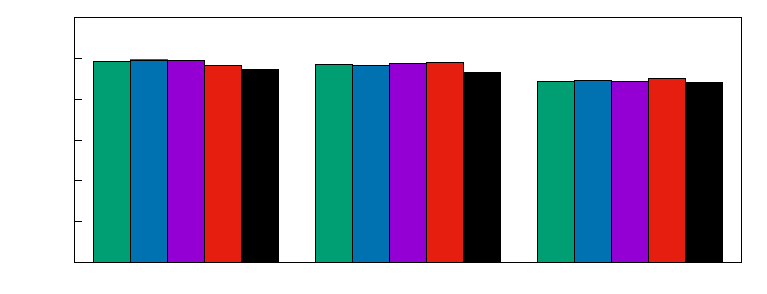
\includegraphics{zif8x-porous-volume}}%
    \gplfronttext
  \end{picture}%
\endgroup

    \caption{Accessible porous volume changes in the three isoreticular
    structures during adsorption. The numbers on top of the columns are the
    number of adsorbed \ce{N2} molecules.}
    \label{fig:zif8x:porous-volume}
\end{figure}

The results presented in figure~\ref{fig:zif8x:pores-sizes} highlight that the
pore size distribution (PSD) remains constant in all cases as the loading
increase and the linkers swing. The PSDs present two cavities: a small one
corresponding to the 6 member windows around \SI{10.3}{\AA} for \ZIF8 and a
second one, with a much larger contribution to the overall porous volume around
\SI{11.2}{\AA} in \ZIF8. The three PSDs are very similar, only changing the size
of pores in the order $\text{\ZIF8} > \text{\ZIFCl} > \text{\ZIFBr}$. This is
also reflected in the accessible volume figure~\ref{fig:zif8x:porous-volume}
which remains roughly constant as the loading increase and the linkers swing.

\subsection{Changes in the adsorbed phase}

In order to understand the origin of the step in the nitrogen adsorption
isotherms, we need to take a look at the other chemical specie participating in
adsorption: the nitrogen fluid. Another hypothesis used to explain the stepped
isotherm is that nitrogen molecules undergoes a reordering or repacking in the
cavity, thereby leading to an increase of adsorbed molecules in the same total
pore volume as well as the swing of the linkers aiming to accommodate the new
packing. This hypothesis had been already proposed by
\citeauthor{Ania2012}\cite{Ania2012}, but the intermediate adsorption regime was
then not probed or interpreted.

In order to visualize this packing, I have projected the positions of all
adsorbed nitrogen atoms in the $xy$ plane and created a density map of the
adsorbed phase. This density map is shown figure~\ref{fig:zif8x:density} both at
various loadings and for the three frameworks.

\begin{figure}[ht]
    \centering
    % % GNUPLOT: LaTeX picture with Postscript
\begingroup
  \makeatletter
  \providecommand\color[2][]{%
    \GenericError{(gnuplot) \space\space\space\@spaces}{%
      Package color not loaded in conjunction with
      terminal option `colourtext'%
    }{See the gnuplot documentation for explanation.%
    }{Either use 'blacktext' in gnuplot or load the package
      color.sty in LaTeX.}%
    \renewcommand\color[2][]{}%
  }%
  \providecommand\includegraphics[2][]{%
    \GenericError{(gnuplot) \space\space\space\@spaces}{%
      Package graphicx or graphics not loaded%
    }{See the gnuplot documentation for explanation.%
    }{The gnuplot epslatex terminal needs graphicx.sty or graphics.sty.}%
    \renewcommand\includegraphics[2][]{}%
  }%
  \providecommand\rotatebox[2]{#2}%
  \@ifundefined{ifGPcolor}{%
    \newif\ifGPcolor
    \GPcolortrue
  }{}%
  \@ifundefined{ifGPblacktext}{%
    \newif\ifGPblacktext
    \GPblacktextfalse
  }{}%
  % define a \g@addto@macro without @ in the name:
  \let\gplgaddtomacro\g@addto@macro
  % define empty templates for all commands taking text:
  \gdef\gplbacktext{}%
  \gdef\gplfronttext{}%
  \makeatother
  \ifGPblacktext
    % no textcolor at all
    \def\colorrgb#1{}%
    \def\colorgray#1{}%
  \else
    % gray or color?
    \ifGPcolor
      \def\colorrgb#1{\color[rgb]{#1}}%
      \def\colorgray#1{\color[gray]{#1}}%
      \expandafter\def\csname LTw\endcsname{\color{white}}%
      \expandafter\def\csname LTb\endcsname{\color{black}}%
      \expandafter\def\csname LTa\endcsname{\color{black}}%
      \expandafter\def\csname LT0\endcsname{\color[rgb]{1,0,0}}%
      \expandafter\def\csname LT1\endcsname{\color[rgb]{0,1,0}}%
      \expandafter\def\csname LT2\endcsname{\color[rgb]{0,0,1}}%
      \expandafter\def\csname LT3\endcsname{\color[rgb]{1,0,1}}%
      \expandafter\def\csname LT4\endcsname{\color[rgb]{0,1,1}}%
      \expandafter\def\csname LT5\endcsname{\color[rgb]{1,1,0}}%
      \expandafter\def\csname LT6\endcsname{\color[rgb]{0,0,0}}%
      \expandafter\def\csname LT7\endcsname{\color[rgb]{1,0.3,0}}%
      \expandafter\def\csname LT8\endcsname{\color[rgb]{0.5,0.5,0.5}}%
    \else
      % gray
      \def\colorrgb#1{\color{black}}%
      \def\colorgray#1{\color[gray]{#1}}%
      \expandafter\def\csname LTw\endcsname{\color{white}}%
      \expandafter\def\csname LTb\endcsname{\color{black}}%
      \expandafter\def\csname LTa\endcsname{\color{black}}%
      \expandafter\def\csname LT0\endcsname{\color{black}}%
      \expandafter\def\csname LT1\endcsname{\color{black}}%
      \expandafter\def\csname LT2\endcsname{\color{black}}%
      \expandafter\def\csname LT3\endcsname{\color{black}}%
      \expandafter\def\csname LT4\endcsname{\color{black}}%
      \expandafter\def\csname LT5\endcsname{\color{black}}%
      \expandafter\def\csname LT6\endcsname{\color{black}}%
      \expandafter\def\csname LT7\endcsname{\color{black}}%
      \expandafter\def\csname LT8\endcsname{\color{black}}%
    \fi
  \fi
    \setlength{\unitlength}{0.0500bp}%
    \ifx\gptboxheight\undefined%
      \newlength{\gptboxheight}%
      \newlength{\gptboxwidth}%
      \newsavebox{\gptboxtext}%
    \fi%
    \setlength{\fboxrule}{0.5pt}%
    \setlength{\fboxsep}{1pt}%
\begin{picture}(7360.00,7360.00)%
    \gplgaddtomacro\gplbacktext{%
    }%
    \gplgaddtomacro\gplfronttext{%
      \csname LTb\endcsname%%
      \put(919,7250){\makebox(0,0){\strut{}\small 10 \ce{N2} $\in$ \ZIFCH3}}%
    }%
    \gplgaddtomacro\gplbacktext{%
    }%
    \gplgaddtomacro\gplfronttext{%
      \csname LTb\endcsname%%
      \put(2759,7250){\makebox(0,0){\strut{}\small 25 \ce{N2} $\in$ \ZIFCH3}}%
    }%
    \gplgaddtomacro\gplbacktext{%
    }%
    \gplgaddtomacro\gplfronttext{%
      \csname LTb\endcsname%%
      \put(4599,7250){\makebox(0,0){\strut{}\small 40 \ce{N2} $\in$ \ZIFCH3}}%
    }%
    \gplgaddtomacro\gplbacktext{%
    }%
    \gplgaddtomacro\gplfronttext{%
      \csname LTb\endcsname%%
      \put(6439,7250){\makebox(0,0){\strut{}\small 50 \ce{N2} $\in$ \ZIFCH3}}%
    }%
    \gplgaddtomacro\gplbacktext{%
    }%
    \gplgaddtomacro\gplfronttext{%
      \csname LTb\endcsname%%
      \put(919,4797){\makebox(0,0){\strut{}\small 10 \ce{N2} $\in$ \ZIFCl}}%
    }%
    \gplgaddtomacro\gplbacktext{%
    }%
    \gplgaddtomacro\gplfronttext{%
      \csname LTb\endcsname%%
      \put(2759,4797){\makebox(0,0){\strut{}\small 25 \ce{N2} $\in$ \ZIFCl}}%
    }%
    \gplgaddtomacro\gplbacktext{%
    }%
    \gplgaddtomacro\gplfronttext{%
      \csname LTb\endcsname%%
      \put(4599,4797){\makebox(0,0){\strut{}\small 40 \ce{N2} $\in$ \ZIFCl}}%
    }%
    \gplgaddtomacro\gplbacktext{%
    }%
    \gplgaddtomacro\gplfronttext{%
      \csname LTb\endcsname%%
      \put(6439,4797){\makebox(0,0){\strut{}\small 50 \ce{N2} $\in$ \ZIFCl}}%
    }%
    \gplgaddtomacro\gplbacktext{%
    }%
    \gplgaddtomacro\gplfronttext{%
      \csname LTb\endcsname%%
      \put(919,2344){\makebox(0,0){\strut{}\small 8 \ce{N2} $\in$ \ZIFBr}}%
    }%
    \gplgaddtomacro\gplbacktext{%
    }%
    \gplgaddtomacro\gplfronttext{%
      \csname LTb\endcsname%%
      \put(2759,2344){\makebox(0,0){\strut{}\small 20 \ce{N2} $\in$ \ZIFBr}}%
    }%
    \gplgaddtomacro\gplbacktext{%
    }%
    \gplgaddtomacro\gplfronttext{%
      \csname LTb\endcsname%%
      \put(4599,2344){\makebox(0,0){\strut{}\small 40 \ce{N2} $\in$ \ZIFBr}}%
    }%
    \gplgaddtomacro\gplbacktext{%
    }%
    \gplgaddtomacro\gplfronttext{%
      \csname LTb\endcsname%%
      \put(6439,2344){\makebox(0,0){\strut{}\small 50 \ce{N2} $\in$ \ZIFBr}}%
    }%
    \gplbacktext
    \put(0,0){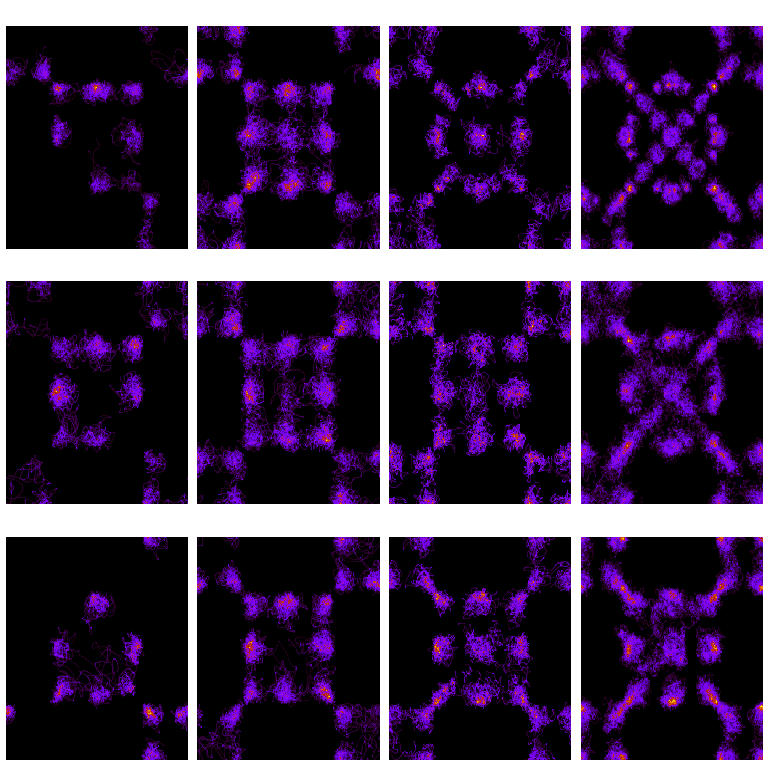
\includegraphics{zif8x-density}}%
    \gplfronttext
  \end{picture}%
\endgroup

    \TODO
    \caption{2D density maps of the adsorbed nitrogen atoms positions in the $xy$
    plane at various loadings in \ZIF8 (top), \ZIFCl (middle), and \ZIFBr
    (bottom). The loading increases from left to right.}
    \label{fig:zif8x:density}
\end{figure}

For \ZIF8, two different molecular packing are encountered according to the
loading. With 10 or 25 molecules in the unit cell, the density maps show clear
delimited positions on a cubic-like arrangement, whereas with 40 and 50
molecules, they show a tetragonal-like arrangement of the molecules. This
reordering of the adsorbed nitrogen molecules from a cubic-like phase to a
tetragonal-like phase is at the origin of the steep uptake at low relative
pressure. For \ZIFCl, the behavior is roughly similar: the molecules first pack
in a cubic-like fashion in the cases of 10, 25 and 40 molecules per unit cell,
before a reordering toward a tetragonal-like arrangement at 50 molecules per
unit cell. This is consistent with the dihedral angles distributions as shown in
figure~\ref{fig:zif8x:dihedrals} and evidences that the molecular packing
rearrangement happens conjointly with the swing of the linkers. It is
interesting to note that some disorder in the tetragonal arrangement remains for
a loading of 50 molecules per unit cell as the molecules positions are not as
well defined as the one in \ZIF8. Again, this is coherent with the dihedral
angles distribution at 50 molecules per unit cell for \ZIFCl which is not of a
single Gaussian type, indicating that this disorder can also be found in the
framework structure. For \ZIFBr, the behavior is different. A same cubic-like
arrangement is found at the lower loadings of 8 and 20 molecules per unit cell,
whereas the arrangement at the higher loadings of 40 and 50 molecules per cell
differ from the tetragonal-like one seen for \ZIF8 and \ZIFCl. Indeed, the
latter appears as a mix of the cubic and the tetragonal organization as the
molecules are mostly distributed on a cube with additional molecules in the
[111] channels on the diagonals of the cube. Consequently, because of the
absence of a neat reordering of adsorbed nitrogen molecules in \ZIFBr, its
sorption isotherm does not display the S-shaped adsorption step.

Given that the change in functional group, and thus in partial atomic charges,
does not significantly impact the strength of the Zn-N coordination bond, we
ascribe the origin of this different sorption feature between the three ZIF-8
derivatives to the difference pore size and shape, the pores in \ZIFBr being
too small to enable a molecular reordering to occur.

\subsection{Conclusion}

\OnlyInSubfile{\printbibliography}

\end{document}
